\section{Stochastic Properties of Random Matrix Factors - 3}

In this third post continuing QR and related Cholesky matrix decomposition techniques, we look at the probability density function (PDF) of a diagonal element of the QR decomposition of a complex-valued random matrix with circular Gaussian i.i.d elements.

Let $\mathbf{H}$ denote an $N\times N$ matrix with circular Gaussian independent and identically distributed (i.i.d) elements with zero mean and variance two i.e. $\mathcal{CN}(0,2)$. Furthermore let $\mathbf{R}$ denote the upper-triangular matrix obtained after QR decomposition ($\mathbf{H} = \mathbf{Q}\mathbf{R}$) such that the diagonal elements of $\mathbf{R}$ are non-negative. It is well-known that such a QR decomposition (QRP or QR with positive diagonal elements) of a matrix is unique. In case a QR decomposition algorithm results in negative diagonal elements, non-negativity may be arranged by multiplying those rows of $\mathbf{R}$ and the corresponding columns of $\mathbf{Q}$ by -1.

It is well known that the diagonal elements of $\mathbf{R}$ follow the distribution:
$$
\begin{bmatrix}
	\chi_{2N} & \mathcal{CN}(0,2) & \cdots &  \mathcal{CN}(0,2)\\
	& \chi_{2(N-1)} & \ddots & \vdots\\
	& & \ddots & \mathcal{CN}(0,2)\\
	& & & \chi_{2}
\end{bmatrix},
$$
where $\chi_{k}$ denotes a Chi-distributed random variable with $k$ degress of freedom.

From the above, it follows that the distribution of a diagonal element $r$ of the matrix $\mathbf{R}$ may be given as the (equal) weighted sum of the pdfs of the diagonal elements as
$$
f_r(x) = \frac{1}{N} \sum_{n=1}^{N} \frac{2^{n}}{\Gamma(n)} x^{n-1} e^{-\frac{x}{2}},
$$
where $\Gamma(n)$ is the Gamma function.

The following graph shows the results of a MATLAB simulation for $N=4$ over 100000 iterations where the diagonal values of $\mathbf{R}$ were collected. The blue graph shows the histogram of the diagonal values. The red graph shows the pdf as obtained using the equation above. We notice that the two correspond well.


\begin{figure}[H]
	\centering
	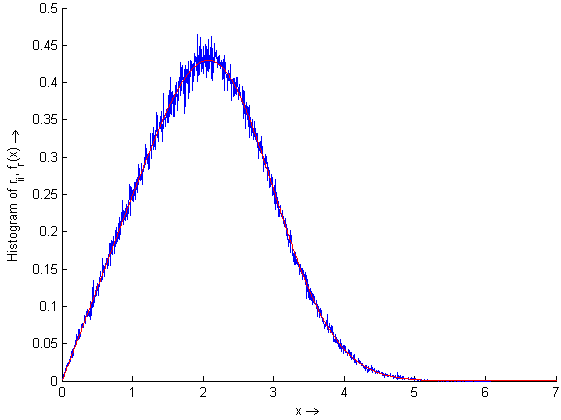
\includegraphics[width=0.5\textwidth,keepaspectratio]{010_001_frx.png}
\end{figure}

ARK

\emph{First published: 29th Dec. 2017 on aravindhk-math.blogspot.com}
